\documentclass[review]{elsarticle}
 
\usepackage[margin=2.5cm]{geometry}
\usepackage{lineno,hyperref,booktabs,multirow,cleveref,pdflscape}
\modulolinenumbers[5]

\journal{Environmental Software and Modeling}

\bibliographystyle{APA-style}\biboptions{authoryear}

\begin{document}

\begin{frontmatter}

\title{Towards Decentralized Integration of Environmental Models on the Web: A Resource Alignment Service}

\author[address1]{Peishi Jiang}
\author[address1]{Mostafa Elag}
\author[address1]{Praveen Kumar\corref{correspondingauthor}}
\cortext[correspondingauthor]{Corresponding author}
\ead{kumar1@illinois.edu}
\author[address2]{Liu Rui}
\author[address2]{Luigi Marini}

\address[address1]{Ven Te Chow, Hydrosystem Laboratory, Civil and Environmental Engineering, University of Illinois, Urbana, IL, USA}
\address[address2]{National Center for Supercomputing Applications, University of Illinois, Urbana, IL, USA}

\begin{abstract}
...
\end{abstract}

\begin{keyword}
decentralized integration \sep web service \sep semantic interoperability \sep the Resource Alignment Service (RAS) 
\end{keyword}

\end{frontmatter}

\linenumbers

\section{Introduction}Integrated environmental modeling is essential in simulating a complex ecosystem \citep{argent2004}. This is because individual scientists or small research groups usually have different practise in modeling in terms of programming language, variable names, units and other factors, causing models from various disciplines hard to be accessed, reused and coupled. Thanks to the advance of web technology, models are able to be exposed as web services (or called as Model as a Service (MaaS)), and integrating these web serviced models over web thus becomes promising \citep{goodall2011}. The traditional integrated modeling approach often requires models to be encapsulated in a specific framework or standard. Meanwhile, coupling models over the web provides an opportunity that models can be independent of any framework or standard by only exposing their functionalities as web services. In this study, we aim to integrate web serviced models in geoscience by utilizing a Resource Alignment Service (RAS), which is able to ensure the semantic consistency of information flowing between web-serviced resources (i.e., model and data).

Traditionally, scientists usually apply a specific framework or standard for coupling their research-required models to tackle the heterogeneity issue of models. To name a few, Community Surface Dynamics Modeling System (CSDMS) \citep{peckham2013}, OpenMI standard \citep{moore2005} and Earth System Modeling Framework \citep{hill2004}. Such tight coupling approach controls both the data structures and processes of all parts of the model. For example, in CSDMS community, each model is wrapped by a BMI (Basic Model Interface) wrapper and coupled with other models under a common framework, as shown in Figure 1(a). The OpenMI provdies a standard\footnote{http://www.opengeospatial.org/node/1822} to convert standalone models into OpenMI-compliant models, and then couples them by using a set of utilities (see Figure 1(b)). Despite of the succesful applications of the tight coupling approach, a factor that cannot be ignored is the difficulty of coupling models that do not follow the same standards or frameworks. There is a need, therefore, to decentralize model integration.

The service-oriented, loose-coupling approach gives the potential to integrate models independent of any framework over the web. Being exposed as web services, models can be conserved in their own hardware environments. As shown in Figure 1(c), the decentralized integration of web serviced models is independent of any integration framework and operating system. Thus, modelers only need to focus on the standardization of the web interface and the protocol of data exchanging \citep{goodall2013}. Web serviced models can ''talk'' to each other if the semantic consistency of quantities exchanged between them is ensured by a utility or web service (e.g., the Resource Alignment Service used in this study).

\begin{figure}[!htbp]
\centering
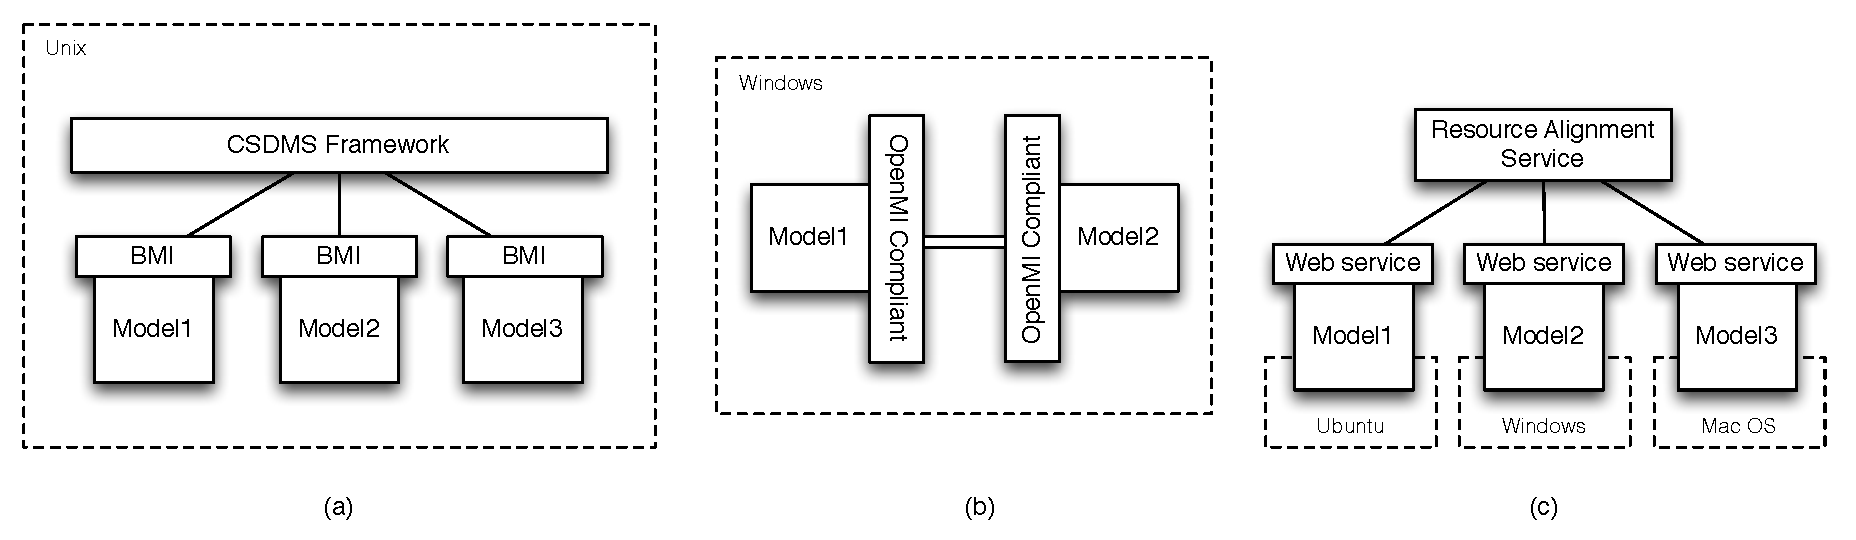
\includegraphics[scale=0.5]{../figures/comparison.pdf}
\caption{A comparison of the traditional tight integration centralized in a specific framework and the decentralized integration through web services. (a) the model integration in CSDMS framework operated in a Unix machine; (b) the integration of OpenMI-compliant models operated in a Windows machine; (c) the decentralized integration of web serviced models operated in various operating system.}
\label{comparison}
\end{figure}

Until recently, the application of the service-oriented architecture in environmental modeling starts \citep{castronova2013, mineter2003, granell2010, goodall2011, goodall2013}. Following the concept of Software as a Service (SaaS), models and data can also be exposed as web services, called as Model as a Service (MaaS) and Data as a Service (DaaS) respectively. \cite{goodall2011} exposed water resource models as web services by using the Open Geospatial Consortium (OGC) Web Processing Service (WPS) and demonstrated how it could be encapsulated as OpenMI-compliant models. Then, \cite{castronova2013} furthered the idea of servicing an OpenMI-compliant model based on WPS by considering the case of time-dependent models. In addition, an OpenMI-ESMF web service wrapper was developed to couple a climate model implemented via ESMF web service with an OpenMI-compliant hydrologic model running on a personal computer \citep{goodall2013}. Furthermore, the concept of ''Model Web'' was put forward to draw the picture of a world of interoperable MaaS and DaaS \citep{geller2007, geller2008}. \cite{nativi2013} then adopted the idea of ''Model Web'' in the Group on Earth Observation (GEO) Model Web initiative. Nevertheless, none of the existing efforts in coupling serviced models, either the application of OpenMI standard in integrating web serviced models or the proposed concept of ''Model Web'', has solved the semantic interoperability issue entirely independent of a modeling integration framework. 

Therefore, in this paper, we develop a web service named Resource Alignment Service (RAS) to ensure semantic consistency of information exchanged between the decentralized web serviced models over the web. The capability of RAS includes (1) semantic mediation between variable names; (2) conversion of mismatched units; (3) temporal alignment of resource time horizon and (4) spatial alignment of resources spatial attributes. Models are implemented by the WPS, which provides an interface standard for exposing both the model execution and the obtain of a model's input(s) and output(s) as web services. Then, RAS is utilized to align the quantities exchanged between the WPS-implemented serviced models.

In the remainder of the paper, Section 2 describes the design requirement of the decentralized integration of web serviced models. In Section 3, the architecture of the Resource Alignment Service (RAS) is presented, including the an brief overview of GeoSemantic framework, the functionality and the components of RAS. Section 4 demonstrates the application of RAS in coupling WPS-implemented models with the input data from Clowder, an online data repository. First we create a workflow of heterogeneous collection of data and WPS-implemented models. Then, we show how RAS can seamlessly align the semantics of quantities exchanging between these resources. Finally, a brief summary is given in Section 5, with mentions on the future work. 

\section{Design Requirement and Overview} A service-oriented architecture is adopted for the decentralized integration of web serviced models. Hence, it is crucial to standardize the communication protocols of web services. In this paper, the OGC Web Processing Service (WPS) specification is implemented for setting up the interface of the serviced models.

\subsection{Background} Service-oriented computing is the application of service-oriented architecture in computation, where models or computing components are distributed on various remote server and provide services to other clients via a communication protocol \citep{huhns2005, erl2004}. The client can be either a user or other web service consuming the functionality exposed over the internet. The service-oriented computing approach implies a loose coupling manner. Following a specific communication protocol, the client makes a request to the web service operating on a remote server over the web. Then, after receiving the request, the service interpretes the incoming information, carries out a certain processing and sends a response back to the client for further application. Based on such architecture, the web serviced models can be conserved in any hardware environment (e.g., operating system) and set up in any programming language. It is also convenient for modelers to maintain and update their models at the backend, without the entire web-based architecture being disturbed. Only the compliance of using a common web service standard and commnication protocol is required for the commnication between client and service successfully.

Written in a certain language (e.g., eXtensive Markup Language (XML) or JavaScript Object Notation (JSON)), the request data needs to follow a specific web service standard. Two common web service standards are the REpresentational State Transfer (REST) specifications and the Simple Object Access Protocol (SOAP). SOAP has been widely applied for setting up web service, usually combined with the Web Service Description Language (WSDL). However, a web service in SOAP/WSDL format is much more complex than a RESTful web service application \citep{mulligan2009}. This is because SOAP is designed for strutured information and therefore requires the incoming data to follow a certain prototype. Meanwhile, a RESTful application only relies on a stateless communication protocol (e.g., the Hypertext Transfer Protocol (HTTP)). By using a set of HTTP methods (GET, POST, PUT, DELETE, HEAD, \cite{fielding1999}), a RESTful application is able to interact with the resources exposed by a web service. In this study, we apply the RESTful application to design our servce-oriented computing for its simplicity and easy-to-use. Nevertheless, due to their general service application, neither SOAP or REST is designed for a specific application (e.g., geoscience). It is also necessary, therefore, to apply a web service standard following REST that is able to define how data is transfered over the web.

In geoscience, much work has been done for the standardization of data transfered between web service. For example, Water Markup Language (WaterML) and the Open Geospatial Consortium (OGC) standards are used for transmitting hydrologic time series data and geospatial data respectively. WaterML is initially applied as the protocol of hydrologic data transmission in WaterOneFlow web services held by Consortium of Universities for the Advancement of Hydrologic Scienc, Inc - Hydrologic Information System (CUAHSI-HIS, \cite{valentine2007}). Now the second version of WaterML is adopted as one of the OGC standards. Furthermore, various types of standards are published by the OGC, which includes but not limited to: (1) specifications for data format such as geography markup language (GML)and keyhole markup language (KML); (2) specifications for data publication such as web coverage service (WCS), web mapping service (WMS) and web feature service (WFS); and (3) specifiations for geoprocessing such as web processing service (WPS).\cite{swain2015} provides a good review of the current open source solutions for water resources web application, most of which apply various OGC standards. In this study, as a geoprocessing standard, OGC WPS is implemented by the web serviced model, which has proven to be successfully applied in other modeling studies requiring data exchanging between services \citep{castronova2013, goodall2011, schaeffer2008,vitolo2012}.

\subsection{Serving models using the OGC WPS specification} The OGC WPS provides an approach for standardizing data processing, including three methods: GetCapabilities, DescribeProcess and Execute. The GetCapabilities method allows clients to receive a list of existing processes or models from the remote server implementing the WPS. The DescribeProcess method replies clients with the metadata of the inputs and outputs of a specific model or process. Finally, the execution of a model or process can be conducted through the Execute method based on the input values from clients. All the three methods can be requested by either HTTP POST or HTTP GET method. In this study, models are implemented by WPS, and we utilized the DescribeProcess and Execute method for retrieving the metadata specifics of the models and the model execution respectively.

PyWPS\footnote{http://pywps.wald.intevation.org/}, a Pythoon package for implementing WPS, is utilized for servicing models. The advantage is that PyWPS provides a module for modeler to apply WPS standard directly on any model. Set up on a specific web server (e.g., Apache\footnote{http://httpd.apache.org/} and Nginx\footnote{http://nginx.org/}), PyWPS is able to expose models as web services applying WPS specification.


\section*{References}

\bibliography{mybibfile}

\end{document}

%%% Local Variables:
%%% mode: latex
%%% TeX-master: t
%%% End:
